% Designed Companion Part IV figure
% Intended for \input{...} beside the matching canonical problem.
\begin{figure}[ht]
\centering
\begin{tikzpicture}[scale=1.05]
  \fill[gray!8] (0,0) circle (2.15);
  \fill[white] (0,0) circle (0.85);
  \draw[thick] (0,0) circle (2.15);
  \draw[thick] (0,0) circle (0.85);
  \draw[dashed] (0,0) circle (1.25);
  \draw[dashed] (0,0) circle (1.65);
  \node[right] at (2.05,0.35) {$U=0$};
  \node[right] at (0.8,-0.35) {$U=1$};
  \node at (0,-2.7) {$U(r)=\dfrac{\log(1/r)}{\log(1/\rho)}$};
\end{tikzpicture}
\caption{After the Möbius normalization, the Dirichlet problem is radial on the annulus. Constant-temperature curves are concentric circles and $U(r)=\log(1/r)/\log(1/\rho)$ interpolates between $1$ at $r=\rho$ and $0$ at $r=1$.}
\label{fig:cp-iv-0124-radial-temperature-annulus}
\end{figure}
